\documentclass[color=usenames,dvipsnames]{beamer}\usepackage[]{graphicx}\usepackage[]{color}
% maxwidth is the original width if it is less than linewidth
% otherwise use linewidth (to make sure the graphics do not exceed the margin)
\makeatletter
\def\maxwidth{ %
  \ifdim\Gin@nat@width>\linewidth
    \linewidth
  \else
    \Gin@nat@width
  \fi
}
\makeatother

\definecolor{fgcolor}{rgb}{0, 0, 0}
\newcommand{\hlnum}[1]{\textcolor[rgb]{0.69,0.494,0}{#1}}%
\newcommand{\hlstr}[1]{\textcolor[rgb]{0.749,0.012,0.012}{#1}}%
\newcommand{\hlcom}[1]{\textcolor[rgb]{0.514,0.506,0.514}{\textit{#1}}}%
\newcommand{\hlopt}[1]{\textcolor[rgb]{0,0,0}{#1}}%
\newcommand{\hlstd}[1]{\textcolor[rgb]{0,0,0}{#1}}%
\newcommand{\hlkwa}[1]{\textcolor[rgb]{0,0,0}{\textbf{#1}}}%
\newcommand{\hlkwb}[1]{\textcolor[rgb]{0,0.341,0.682}{#1}}%
\newcommand{\hlkwc}[1]{\textcolor[rgb]{0,0,0}{\textbf{#1}}}%
\newcommand{\hlkwd}[1]{\textcolor[rgb]{0.004,0.004,0.506}{#1}}%
\let\hlipl\hlkwb

\usepackage{framed}
\makeatletter
\newenvironment{kframe}{%
 \def\at@end@of@kframe{}%
 \ifinner\ifhmode%
  \def\at@end@of@kframe{\end{minipage}}%
  \begin{minipage}{\columnwidth}%
 \fi\fi%
 \def\FrameCommand##1{\hskip\@totalleftmargin \hskip-\fboxsep
 \colorbox{shadecolor}{##1}\hskip-\fboxsep
     % There is no \\@totalrightmargin, so:
     \hskip-\linewidth \hskip-\@totalleftmargin \hskip\columnwidth}%
 \MakeFramed {\advance\hsize-\width
   \@totalleftmargin\z@ \linewidth\hsize
   \@setminipage}}%
 {\par\unskip\endMakeFramed%
 \at@end@of@kframe}
\makeatother

\definecolor{shadecolor}{rgb}{.97, .97, .97}
\definecolor{messagecolor}{rgb}{0, 0, 0}
\definecolor{warningcolor}{rgb}{1, 0, 1}
\definecolor{errorcolor}{rgb}{1, 0, 0}
\newenvironment{knitrout}{}{} % an empty environment to be redefined in TeX

\usepackage{alltt}
%\documentclass[color=usenames,dvipsnames,handout]{beamer}

\usepackage[sans]{../lab1}
\usepackage[hang,flushmargin]{footmisc}


\hypersetup{pdftex,pdfstartview=FitV}






%% New command for inline code that isn't to be evaluated
\definecolor{inlinecolor}{rgb}{0.878, 0.918, 0.933}
\newcommand{\inr}[1]{\colorbox{inlinecolor}{\texttt{#1}}}


\title[slides]{Some thoughts on experimental design and
  graduate student research}
\author{Richard Chandler \\ Based on presentation by Dr. Bob Cooper}
\date{September 9, 2021}
\IfFileExists{upquote.sty}{\usepackage{upquote}}{}
\begin{document}


\begin{frame}[plain]
  % \maketitle
  \centering
  \LARGE
  Some Thoughts on Experimental Design and Graduate Student Research \\
  \vfill
  \large
  Richard Chandler \\
  (Based on presentation by Dr. Bob Cooper) \\
  Warnell School of Forestry and Natural Resources \\
  September 9, 2021
\end{frame}



\begin{frame}
  \frametitle{Outline}
  
\end{frame}


\section{Background}

\begin{frame}
  \frametitle{Terminology}
  {\bf Experimental Design:} \\
  The logical structure of an experiment \\ %(Fisher 1971) \\
  \vfill  
  Includes:
  \begin{itemize}
    \item Type of experimental units employed
    \item Number of treatment types (including controls)
    \item Response variables measured
    \item Manner in which treatments are applied
    \item Number of experimental units receiving each treatment (replicates)
    \item Physical and temporal arrangement of experimental units
    \item Controlling extraneous sources of variability, etc.
  \end{itemize}
  \vfill
  \vspace{6pt}
  \rule[0mm]{1cm}{0.1mm} \\
  \footnotesize
  Fisher, R.A. (1971) The Design of Experiments. Macmillan. 
\end{frame}



\begin{frame}
  \frametitle{More terminology} 
  {\bf Experiment} \\
  An act or operation for the purpose of discovering something unknown \par
  \vspace{6pt}
  {\bf Experimental unit} \\
  The unit to which the treatments are applied \par
%  \vfill
  \vspace{6pt}
  {\bf Mensurative experiment} \\
  An experiment that involves only the making of measurements at one
  or more points in space or time. (a.k.a. observational study) \par
%  \vfill
  \vspace{6pt}
  {\bf Manipulative experiment} \\
  An experiment in which the different experimental units receive
  different treatments and the assignment of the treatments is or can
  be randomized. \\
  \vfill
  \vspace{6pt}
  \rule[0mm]{1cm}{0.1mm} \\
  \footnotesize
  Hurlbert, S.A. (1984) Pseudoreplication and the design of ecological field
  experiments.  Ecological Monographs 54:187-211.
\end{frame}



\begin{frame}
  \frametitle{The Scientific Method}
  \begin{enumerate}[1.]
    \item State the problem
    \item Formulate the hypothesis
    \item Design the experiment or observational study
    \item Make observations
    \item Analyze data
    \item Draw conclusions
    \end{enumerate}
\vfill    
\centering    
Where does statistical analysis fit in?  Where do most courses in
statistics apply to the scientific method? \\
\vfill
Where does experimental design fit in?  Courses? \\
\end{frame}

\section{Experiments}


\begin{frame}
  \frametitle{Example: Timber harvest and salamanders}
  Suppose we wish to assess the effect of timber harvest on salamander
  abundance.  One plot is established in each of two forests, one
  thinned and the other untreated, in which we trap salamanders at n=9
  pitfall traps.  The response variable of interest is the number of a
  species captured per trap.  The explanatory variable is silvicultural
  treatment. \\
  \vfill
  \centering
  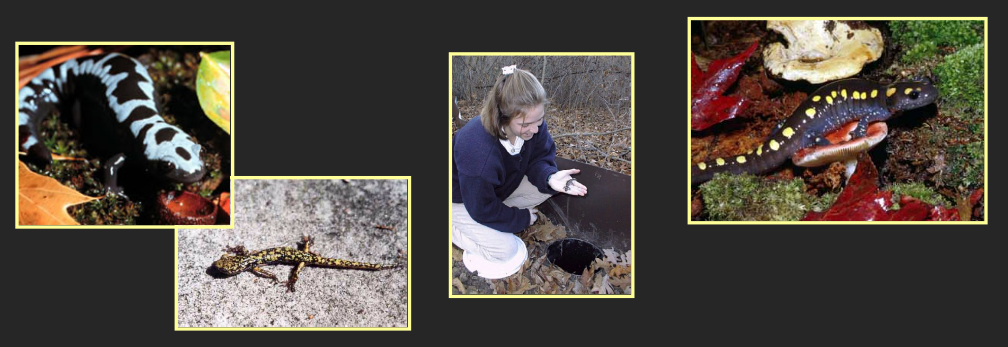
\includegraphics[width=\textwidth]{salamanders} \\
\end{frame}


\begin{frame}
  \frametitle{Example: Timber harvest and salamanders}
  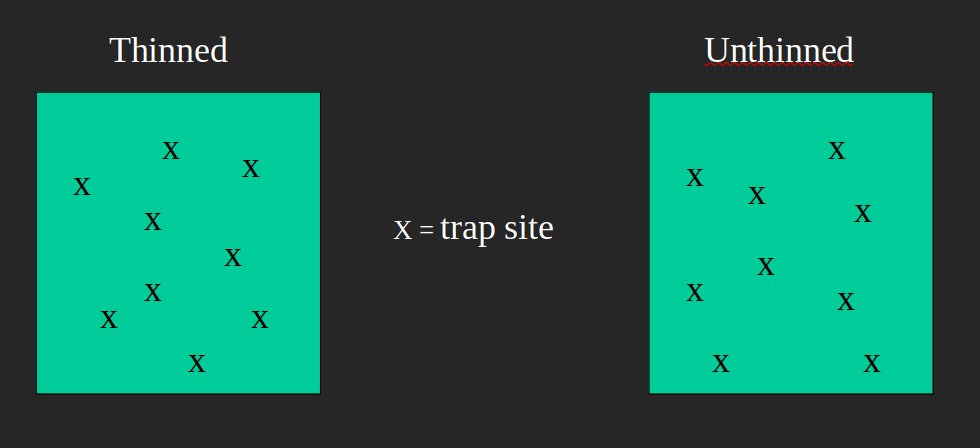
\includegraphics[width=\textwidth]{salamander-design} \\
  \vfill
  The response variable of interest is the number of red-backed
  salamanders captured per trap.  The explanatory variable is harvest
  treatment (thinned/not). We find more salamanders on the untreated
  plot, and conclude that thinning is bad for salamanders.  What is
  wrong with this design?  
\end{frame}


\begin{frame}
  \frametitle{Example: Timber harvest and salamanders}
  Problems
  \begin{itemize}
    \item Unreplicated
    \item Confounding of sources of variation -- is the
      difference due to treatment or location or some other unmeasured
      variable?
    \item Pseudoreplication -- use of the incorrect (higher) error
      degrees of freedom in a statistical test. 
  \end{itemize}
\end{frame}



\begin{frame}
  \frametitle{Features of good experimental design}
  {\bf Replication} \\
  More than one experimental unit or replicate per treatment. Allows
  one to estimate experimental error (variability among experimental
  units). 
  \vfill
  {\bf Randomization} \\
  All units must have an equal chance of receiving all treatments.
  Otherwise, estimates may be biased.  Depends on a mechanical
  process. 
  \vfill
  {\bf Controls} \\
  Allows one to isolate the causative agent of interest (treatment
  effect).  Not always an untreated treatment. 
  \vfill
  {\bf Interspersion} \\
  Hurlbert's recommendation that treatments be spatially interspersed.  
\end{frame}


\begin{frame}
  \frametitle{Various designs}
  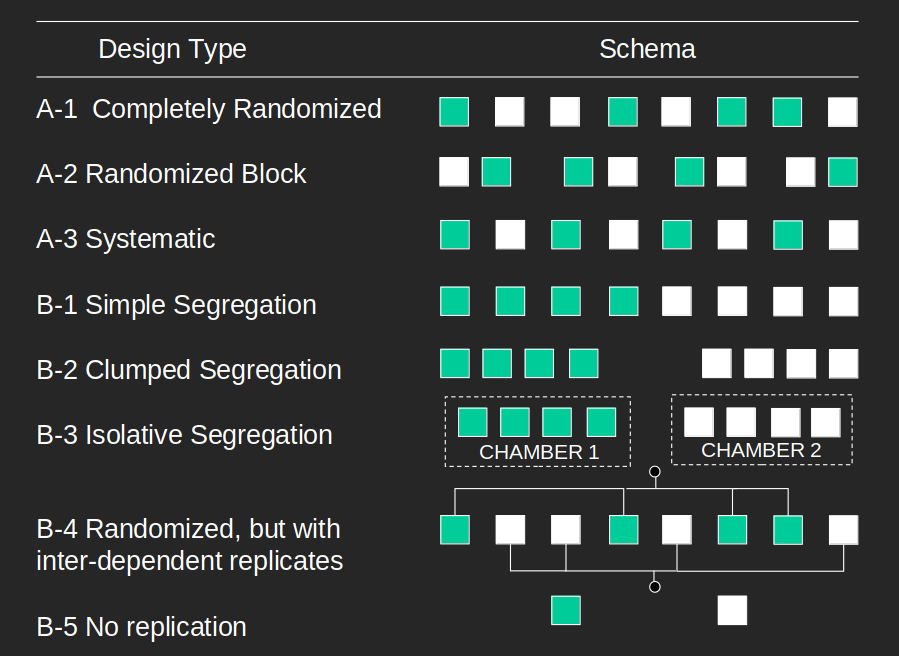
\includegraphics[width=\textwidth]{Hurlbert-schema} \\
  \centering
  From Hurlbert (1984) \\
\end{frame}



\begin{frame}
  \frametitle{Example 2: Factors that affect growth and survival of
    tree seedlings in a bottomland forest}
  Suppose we wish to understand the factors that influence growth and
  survival of tree seedlings in a periodically flooded bottomland
  forest.  Depending on our objectives (and prior knowledge), we might
  take several approaches to address this topic. \\

  Option 1: Observation study -- measure factors (variables) {\it in
    situ} that you think will influence growth and survival of seedlings. 
	(a) controlling and manipulating nothing
	(b) examining correlations between growth of seedlings and the variables
	(c) modeling: finding the best model from a candidate
        set. Ideally, the models should be predictive and mechanistic
        (based on theory).


  Option 2: Manipulative experiment -- focus on a few key variables of
  particular interest and attempt to hold all else constant. 
	(a) e.g., manipulate shading and flooding (plus interactions) in a greenhouse setting.
	(b) other factors (soil, herbivory, etc.) held constant.
	(c) features of good experimental design still needed, even in
        a highly controlled laboratory and greenhouse setting. 
	(d) cause and effect can be established in the greenhouse –
        extrapolation to a field setting?         
\end{frame}



\begin{frame}
  \frametitle{Example 3: Effect of effluent from a new power plant on
    fish species richness in a river}
  A new power plant is to be established along the Oconee River.  We
  know for several years beforehand that the plant will be built.  So
  a survey is designed where fish are sampled periodically above
  (upriver from) and below (downriver from) the site, with repeated
  surveys done before and after the plant goes on line.  These are
  then compared to assess the effect of the plant on species richness.   
\end{frame}


\begin{frame}
  \frametitle{Example 3: Effect of effluent from a new power plant on
    fish species richness in a river}
  \centering
  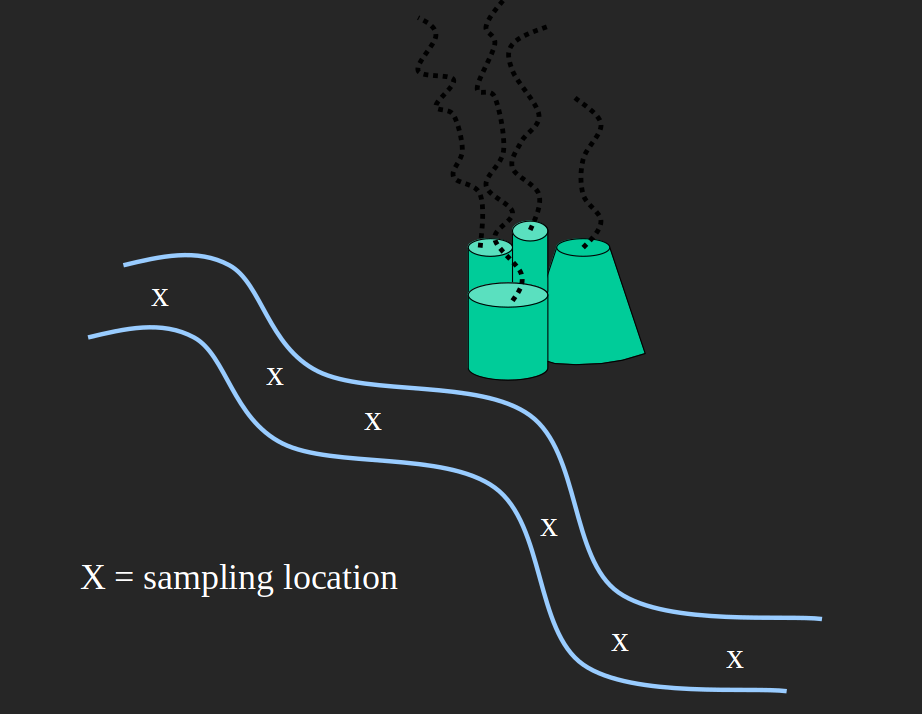
\includegraphics[width=\textwidth]{power-plant-river} \\
\end{frame}


\begin{frame}
  \frametitle{Example 3: Effect of effluent from a new power plant on
    fish species richness in a river}
  \centering
  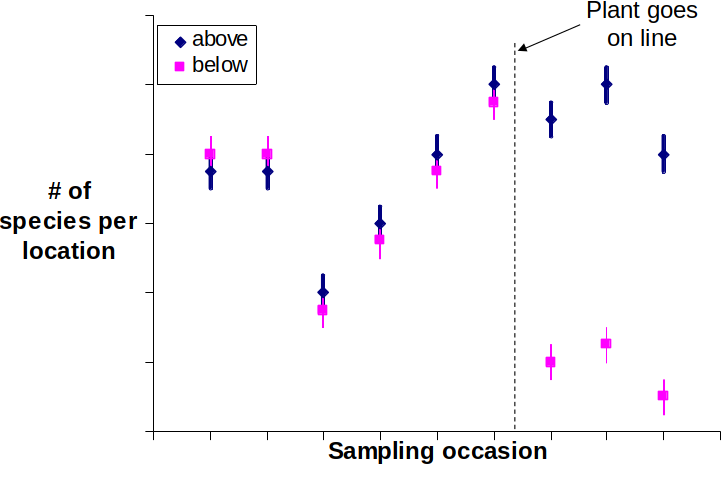
\includegraphics[width=\textwidth]{power-plant} \\
\end{frame}


\section{Observational Studies}


\begin{frame}
  \frametitle{Observational studies}
  Are (properly designed) manipulative experiments better than
  observation studies?

  Yes, correlation does not imply causation. But, manipulative
  experiments aren't always possible or necessary. 

  Extensive, ongoing research on methods for causal inference in
  observational research.
  
\end{frame}


\begin{frame}
  \frametitle{Conclusions}
  What does this mean for graduate student research?
  \begin{itemize}
    \item Graduate students only have a couple of years to create an
      interesting question, design a study to address that question,
      collect and analyze data, and write a thesis.
    \item Long-term study usually out of the question.
    \item Focus on a particular question in a
      broader framework.
    \item Often, students are handed a thesis topic. Pros and cons.
    \item Manipulative experiments make for stronger
      inference but are not always appropriate or possible.
    \item Observational studies are fine -- consider
      developing predictive models based on hypotheses.
  \end{itemize}
\end{frame}


\end{document}
